% Chapter 2

\chapter{Literature Background} % Write in your own chapter title
\label{Chapter2}
\lhead{Chapter 2. \emph{Literature}} % Write in your own chapter title to set the page header

\section{Introduction}

In trying to make sense of what to write in this Literature Review, and thrashing around for a bit, I discovered Randolph's paper \cite{Randolph2009}, which contains Table~\ref{tab:TaxonomyOfLiteratureReview}. While Randolph's and Cooper's papers are written for an audience of social scientists I think it is a worthwhile paper to follow for in my experience social scientists are much more rigorous in researching their research questions than natural scientists. 

I think it will be of assistance to the reader if I explain what to expect in the review, and why.

The \emph{focus} of the rewiew will be on ``practices or applications'', since our goal is to develop practical new instrumentation. 

It's \emph{goal} will be the ``identification of central issues'', because we want to discover what new direction we want to go in and how our technologies fit into the whole.

The \emph{perspective} will be a ``neutral representation''. As is the custom in quantitative research such as analytical chemistry we will neutral perspective and strive to present our findings as facts.

The \emph{coverage} will be ``central or pivotal''. The coverage will not be exhaustive, but central, to point the reader to the main findings in literature. The literature is littered with papers that describe the production of biodiesel from various oils and fats, and its testing in an engine. 

The \emph{organization} will be ``conceptual'' with some ``historical'' context. 

The \emph{audience} will be ``specialized scholars''. The primary audience are the examiners, and the secondary audience are the students following me. 

\begin{table}
\caption{Cooper�s \cite{Cooper1988} Taxonomy of Literature Reviews}
\centering

\begin{tabular}{|l|l|}
\hline
Characteristic & Categories\\
\hline
Focus &	 Research outcomes \\
 & Research methods \\
 & Theories \\
 & Practices or applications \\
\hline
Goal & Integration \\
 & (a) Generalization \\
 & (b) Conflict resolution \\
 & (c) Linguistic bridge-building \\
 & Criticism \\
 & Identification of central issues \\
\hline
Perspective & Neutral representation \\ 
 & Espousal of position \\
\hline
Coverage & Exhaustive \\
 & Exhaustive with selective citation \\ 
 & Representative \\
 & Central or pivotal \\
\hline
Organization & Historical \\
 & Conceptual \\
 & Methodological \\
\hline
Audience & Specialized scholars \\
 & General scholars \\
 & Practitioners or policymakers \\
 & General public \\
\hline
\end{tabular}

\end{table}
\label{tab:TaxonomyOfLiteratureReview}
\section{GC}

Knothe (2006) \cite{Knothe2006} has written a review on the analysis of biodiesel, explaining the origin of biodiesel. The main standards 
for the analysis of biodiesel are based on GC.

The analysis of fatty acids predates biodiesel, of course, because of the use in the food industry, where the fatty acids are converted to FAMEs to make it amenable to analysis by gas chromatography.

The most problematic contaminants of biodiesel are glycerol and the acyl glycerides. These are determined by a procedure developed by Plank and Lorbeer \cite{Plank1995}. It involves derivitization of the free glycerol and acyl glycerides by silylation, using MSTFA (N-Methyl-N-trimethylsilyltrifloroacetamide.) This reagent reacts with the free hydroxyl groups on the free glycerol and glycerides, leaving it with a nonpolar trimethylsilyl group on the oxygen. (Figure~\ref{fig:Silylation}) This lowers the elution temperature of the compound and makes it less likely to interact with active sites on the system, thereby improving peak shapes.

\begin{figure}[htbp]
	\centering
	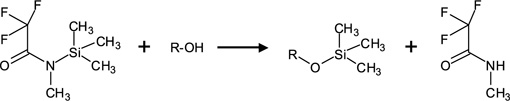
\includegraphics[width=0.8\textwidth,natwidth=4.17in,natheight=3.32in]{./Figures/silylation.jpg}
	\rule{35em}{0.5pt}
	\caption[A silylation reactio]{The silylation reaction to facilitate the chromatography of glycerides.}
	\label{fig:Silylation}
\end{figure}

\section{\texorpdfstring{\GCxGC}{GCxGC}}

Comprehensively coupled \GCxGC has been used to analyse biodiesel.

\section{SFC}

Supercritical fluid chromatograpy was invented by Klesper e.a. in 1962 \cite{} using CFCs, altough the first mention of the phrase `supercritical fluid' found by the indexing service Scopus is a paper by Sie and Rinders in 1967, who used carbon dioxide. According to Saito (one of the oldest workers in this field) \cite{Saito2013} or cite (jp.linkedin.com/pub/muneo-saito/17/500/30) it developed somewhat, but in the 1980s capillary column supercritical fluid chromatography appeared and was oversold, which confused users about the use and potentials of SFC. During the 1990s some applications for SFC appeared, and it found a solid niche in the pharmaceutical industry.

First work experimented with various substances (SF6) above their supercritical points, but the low price, inertnes, non-toxicity and reasonable critical point (37 degC at 7.38MPa) made carbon dioxide the universal mobile phase for SFC today. 

SFC with FID detection had the wonderful feature that it was a universal mass sensitive detector.

SFC with MS: what are the problems. Solvable with GC very well known. 

We are much encouraged by the introduction or commercial instrumentation, such as the Waters UPC2 system. 

\section{LC}

According to the review of Pauls \cite{Pauls2011} LC methods for the analysis of biodiesel are growing and "liquid chromatographic methods are beginning to gain favor and are likely to become more widely utilized with improvements in detector technology." 

Of particular interest to our work are the normal phase LC procedures reported. As a rough rule of thumb, supercritcal carbon dioxide has the solubility of dichloromethane, so that using supercritical carbon dioxide with a silica column is approximately like doing normal phase liquid chromatography. 

The use of silver ions in stationary phases to separate 

\section{HPLC-GC}



\section{Miscellaneous}	

In the early enthusiasm for biodiesel much was said about the benefit that biodiesel could have for countries and regions with little money but agricultural potential. If one assumes that biodiesel would be produced locally and not the oil simply exported, the question arises about what one can do about quality control without expensive LC and/or GC equipment. One answer is the use of more traditioal methods of wet chemsitry. Pisarello \cite{Pisarello2010} suggests a titrimetric method, which requires no expensive instrumentation. An examination of the citing papers show that, eight of the nineciting papers were in the field of biodiesel production. The exception was a review paper. 

\section{Techniques similar to \SFCxGC}
	\subsection{SFC-GC}
	Fractions of SFC can be collected. 
	\subsection{\SFCxSFC}
	The Japanese used SFCxSFC to analyze trigycerides \cite{Hirata2003}and FAMEs \cite{Hirata2004} using \SFCxSFC. 